\chapter{Propositielogica}\label{ch:proposities}
Als men wil gaan redeneren, dan is het belangrijk dat er bij de overdracht van een redenatie geen verandering ontstaat van hetgeen waarover men aan het redeneren is. Om ervoor te zorgen dat er geen misverstanden ontstaan over hetgeen dat iemand probeert uit te drukken, of de ander van te overtuigen, dient men te beschikken over een arsenaal van begrippen en uitdrukkingswijzen. Alleen wanneer men over deze zaken tot overeenstemming kan komen, bestaat er een redelijke kans dat twee of meer beoefenaars van een vak met elkaar kunnen praten zonder al te vaak in onzekerheid te verkeren over de betekenis van mededelingen die worden uitgewisseld.

Natuurlijke taal (dagelijkse spreektaal, zoals Nederlands of Engels) voldoet op dit vlak helaas niet, omdat natuurlijke taal niet precies genoeg is om verschillende interpretaties uit te sluiten. Een paar voorbeelden van zinnen die men in de krant zou kunnen lezen:
\begin{quote}
\enquote{niemand kan dit bijna doen}
\end{quote}
\begin{quote}
\enquote{kamer aangeboden voor student, tot 25 jaar}
\end{quote}
\begin{quote}
\enquote{wegens lekkage kerncentrale gesloten}
\end{quote}

Er bestaat in bovenstaande voorbeelden weinig kans op misverstanden omdat verkeerde (?) interpretatie onwaarschijnlijke situaties schetst. Echter\ldots het laatste bericht zou ook op de deur van een winkel kunnen hangen. En het is menigmaal voorgekomen dat een verdachte vrijgesproken is op grond van een onduidelijk gestelde beschuldiging.

Voorbeelden van een \enquote{vaktaal} in andere disciplines vinden we heel duidelijk in de protocollen van gerechtelijke uitspraken, en in notari\"ele akten. Ook daar heeft men gekozen voor bepaalde vaste formuleringen om de zaken ondubbelzinnig vast te leggen. Voor een buitenstaander wordt het daardoor echter meestal niet duidelijk, vaak is juist het tegendeel het geval!

De manier waarop iets is opgeschreven valt onder het begrip \textit{syntax}, de betekenis van het opgeschrevene valt onder het begrip \textit{semantiek}. We kunnen dus zeggen dat \enquote{zeven} en \enquote{7} syntactisch verschillend en semantisch hetzelfde zijn. Hier introduceren wij eerst de syntax van de propositielogica, de semantiek volgt later in sectie \ref{sec:wtab}.

\begin{aside}[Syntax vs. semantiek: De Jabberwocky]\mbox{}\\
Schrijver en logicus Lewis Carroll (1832 -- 1898) was erg geinteresseerd in de fenomenen taal en logica. Het is ook niet verwonderlijk dat hij in meerdere van zijn boeken logische puzzels verstopte en de relaties tussen taal en logica onderzocht.

E\'en zo'n voorbeeld is het Jabberwocky nonsensgedicht uit \textit{Through the Looking Glass, and What Alice Found There}, het vervolg op beroemde \textit{Alice's Adventures in Wonderland} \cite{carroll}. Carroll speelt hierin met het correct formuleren van taal (\emph{syntax}) en het cre\"eren van nonsense in betekenis (\emph{semantiek}). \\[2.5pt]

Engels origineel \cite{carroll}:
\begin{quote}
    'Twas brillig, and the slithy toves\\
    Did gyre and gimble in the wabe:\\
    All mimsy were the borogoves,\\
    And the mome raths outgrabe.
\end{quote}
Nederlandse vertaling\\ \cite{wauwelwok}:
\begin{quote}
    't Wier bradig, en de spiramants\\
	Bedroorden slendig in het zwiets:\\
	Hoe klarm waren de ooiefants,\\
	Bij 't bluifen der beriets.\\
\end{quote}

  \begin{marginfigure}
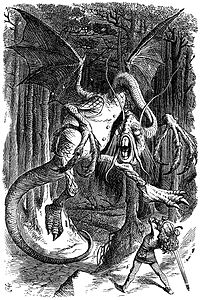
\includegraphics[width=0.6\textwidth]{jabberwocky.jpg}\\
   De Jabberwocky {\scriptsize\emph (Image by Wikipedia)}\\[3mm]
  \end{marginfigure}

Terwijl het gedicht in eerste oogopslag op een correct geformuleerd (Nederlands/Engels) gedicht lijkt, staat er in wezen niks dat betekenis vol is; alle woorden zijn correct gevormd (volgens fonetisch taalregels), maar hebben geen duidelijke betekenis\footnote{Het gedicht is nog briljanter omdat het door gebruik van onomatopees (klanknabootsingen) alsnog een boodschap weet over te brengen.}.
\end{aside}

Om het benodigde begrippenapparaat te introduceren om binnen de informatica (en wiskunde) precies te kunnen beschrijven wat er bedoelt wordt introduceren we nu het belangrijkste begrip van dit hoofdstuk.
\begin{definition}[Propositie]\label{def:prop}\mbox{}\\
Een \textit{propositie} is een zinvolle bewering, een vaststelling met een duidelijke betekenis: \textit{waar} \'of \textit{niet waar}.
\end{definition}

Het is erg lastig om een fundamenteel begrip zoals \enquote{propositie} ondubbelzinnig vast te leggen. Hoe objectief zijn \enquote{zinvol} en \enquote{duidelijk}? Wanneer we ons beperken tot de beweringen in een programmeertaal, dan is het tamelijk eenvoudig om precies te defini\"eren wat een propositie is, dat wil zeggen: hoe een propositie er syntactisch uitziet. We hebben dan wel een beperkte woordenschat, en kunnen gebruikmaken van de syntactische schema's die de programmeertaal defini\"eren. Wij zullen ons hier echter niet zo strikt vastleggen op de syntax, omdat we de theorie toepasbaar willen laten zijn op algemene onderwerpen uit wiskunde \`en informatica.

Voorbeelden van proposities zijn:
\begin{quote}
\begin{tabular}{p{.4\textwidth}p{.4\textwidth}}
\multicolumn{2}{l}{\enquote{in deze zaal zitten 140 mensen}}\\
\enquote{een plus een is twee}&\enquote{drie plus vijf is zes}\\
\enquote{de maan is een spiegel}&\enquote{$3+5=6$}\\
\enquote{dit bewijs is fout}&\enquote{$1-1=0$}
\end{tabular}
\end{quote}

We laten nu een paar voorbeelden zien van uitspraken die geen proposities zijn, en geven bij iedere uitspraak een kort commentaar tussen haakjes:
\begin{quote}
\begin{tabular}{p{.3\textwidth}p{.5\textwidth}}
\enquote{$x$ is gelijk aan $y$}&(niet duidelijk wat $x$ is en wat $y$ is)\\
\enquote{ga naar huis}&(geen vaststelling, maar een bevel)\\
\enquote{zou het regenen?}&(vragen zijn niet waar of onwaar; wel goed is \enquote{het regent})\\
\enquote{Jan te ver kaas}&(wat zou hiervan de betekenis zijn? Dit voldoet ook niet aan de syntax van de Nederlandse taal)
\end{tabular}
\end{quote}

Tenslotte nog een paar voorbeelden van uitspraken die wat complexer van aard zijn, en daarom meer aandacht vragen als het gaat om de vraag of het proposities zijn:
\begin{quote}\label{q:non:prop}
\enquote{alle mensen zijn dieren}\\
\enquote{als het gras nat wordt, dan regent het}\\
\enquote{Jan is een zoon van Kees en Mien is de moeder van Jaap}\\
\enquote{de zon schijnt of het regent}
\end{quote}

Een nieuwe element in bovenstaande uitspraken is dat er verschillende beweringen in \'e\'en uitspraak worden gedaan. We komen later hierop terug in sectie \ref{sec:samenstelling}.

In enkele van de voorbeelden zien we dat een propositie niet waar hoeft te zijn. In de definitie van het begrip propositie (definitie \ref{def:prop}) hebben we ge\"eist dat hij hetzij \textit{waar} hetzij \textit{onwaar} is (precies \'e\'en van beide). Dit betekent echter niet dat we over de waarheid onmiddellijk uitsluitsel moeten kunnen geven. Zo beschouwen we de uitspraak
\begin{quote}
\enquote{onder de eerste tien miljard decimalen van $\pi$ komen precies \'e\'en miljard cijfers $9$ voor}
\end{quote}
wel als een proposities. Immers, zij is waar of onwaar, maar we kunnen (nog) niet vaststellen of zij waar danwel onwaar is. Daarentegen is
\begin{quote}
\enquote{deze zin is onwaar}
\end{quote}
geen propositie. Immers, deze bewering kan niet waar zijn (want dan zegt zij zelf onwaar te zijn) en zij kan ook niet onwaar zijn (want dan zegt zij zelf waar te zijn). Men kan ook zeggen dat deze bewering zowel waar als onwaar is, maar naar onze begrippen is de betekenis van deze bewering niet duidelijk.

Merk op dat we gebruik hebben gemaakt van een nog onuitgesproken afspraak, die we nu expliciet zullen vastleggen.
\begin{axiom}\label{ax:dubbel}
\enquote{niet onwaar} betekent hetzelfde als \enquote{waar}.
\end{axiom}
Dit axioma (een fundamentele afspraak) is een hoeksteen van de klassieke logica. Hierdoor wordt het mogelijk om een bewijs uit het ongerijmde te vormen: als de ontkenning van de propositie onwaar is, dan is de propositie zelf waar!

\begin{aside}[Constructieve logica]\mbox{}\\[1em]
Niet alle filosofen zijn het eens over het gebruik van axioma \ref{ax:dubbel} in de klassieke logica. De Nederlandse filosoof en wiskundige Luitzen Brouwer formuleerde een logica, \textit{intu\"itionistische logica}, waarin dit axioma niet als uitgangspunt werd genomen (sterker nog, in intu\-\"itionistische logica is de propositie die wordt uitgedrukt door axioma \ref{ax:dubbel} niet te bewijzen en dus onwaar).

  \begin{marginfigure}
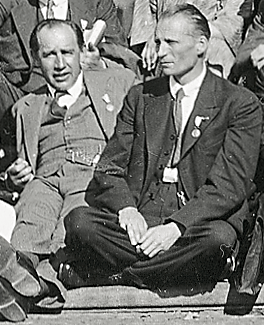
\includegraphics[width=0.6\textwidth]{Bohr_Brouwer.png}\\
    Luitzen Brouwer (rechts) {\scriptsize\emph (Image by Wikipedia)}\\[3mm]
  \end{marginfigure}
 
\hspace{15pt}Intu\"itionistische logica wordt gerekend tot de stroming van het \textit{constructivisme} (of constructieve wiskunde), omdat voor elk stelling een bewijs moet worden gemaakt (geconstrueerd); d.w.z., een stelling is alleen `waar' als er bewezen kan worden dat deze waar is. Het gebruik van bewijzen uit het ongerijmde (waarmee men bewijst dat een stelling `waar' is door te bewijzen dat zijn ontkenning `onwaar' is) is niet toegestaan.

Intu\"itionistische logica wordt veelal toegepast in de correctheid bewijzen van algoritmes binnen de informatica.
\end{aside}

% In het vervolg zullen we de betekenis van een propositie vernauwen tot het waar danwel onwaar zijn van de propositie.
In het vervolg zullen we met de betekenis van een propositie bedoelen of deze waar of onwaar is.

\section{Samenstellen van proposities}\label{sec:samenstelling}
Het kunnen opschrijven van proposities die waar danwel onwaar zijn geeft ons een krachtige basis, maar we willen ook kunnen redeneren over combinaties. Zoals in sommige voorbeelden al te zien was (zie pagina \pageref{q:non:prop}) is het wenselijk dat we proposities kunnen samenstellen. Wat we zouden willen is dat zo'n samenstelling zelf ook weer een propositie zou worden. Daarvoor is nodig dat de samenstelling ook voldoet aan de definitie van propositie (definitie \ref{def:prop}), en dus moeten we precies vastleggen wat we bedoelen met uitspraken als
\begin{quote}
\enquote{\ldots en \ldots}\\
\enquote{\ldots of \ldots}\\
\enquote{als\ldots dan\ldots}\\
\enquote{\ldots dan, en slechts dan, als\ldots}\\
\enquote{niet \ldots}
\end{quote}
waarin op de plaats van de stippeltjes proposities kunnen  worden ingevuld.

Een eerste stap in het vastleggen van een notatie voor deze samenstellingen. Het is niet verstandig om hiervoor alleen het gewone woordgebruik te kiezen. Immers, aan het begin van dit hoofdstuk hebben we al gezien dat hierdoor misverstanden kunnen ontstaan bij de interpretatie. Daarnaast heeft het invoeren van een compacte notatie het voordeel dat ingewikkeldere uitdrukkingen die we daarmee kunnen opbouwen, nog steeds betrekkelijk compact opgeschreven kunnen worden.
\begin{notation}\mbox{}\\
Laten $p$ en $q$ proposities voorstellen. We gebruiken de volgende notaties:\\

  \noindent\parbox{2cm}{$p\land q$} voor \enquote{$p$ en $q$}\\
  \noindent\parbox{2cm}{$p\lor q$} voor \enquote{$p$ of $q$}\\
  \noindent\parbox{2cm}{$p\rightarrow q$} voor \enquote{als $p$ dan $q$} of \enquote{$q$ als $p$}\\
  \noindent\parbox{2cm}{$p\leftrightarrow q$} voor \enquote{$p$ dan, en slechts dan, als $q$}\sidenote{De uitspraak \enquote{$p$ dan en slechts dan als $q$} wordt vaak afgekort tot \enquote{$p$ desda $q$} of \enquote{$p$ iff $q$} (naar het Engels: \enquote{$p$ if and only if $q$}).}\\
  \noindent\parbox{2cm}{$\neg p$} voor \enquote{niet $p$}\\


\noindent
De symbolen $\land$, $\lor$, $\rightarrow$, $\leftrightarrow$, $\neg$ heten \textit{connectieven}, of ook wel \textit{Boolse operatoren}. Ze staan respectievelijk bekend onder de namen \textit{conjunctie}, \textit{disjunctie}, \textit{implicatie}, \textit{bi-implicatie} en \textit{negatie}.
\end{notation}

\subsection{Opgaven}
\begin{exercise}[Proposities]\mbox{}\\
Welke van de volgende uitspraken is een propositie en welke niet?
\begin{enumerate}[label=\textit{\alph*.}]
\item $7+7 = 13$.
\item $7+7 = 14$.
\item Er bestaan groene koeien.
\item Er bestaat leven op een andere planeet.
\item Het schilderij \textit{De Nachtwacht} van Rembrandt is mooi.
\item Koning Willem-Alexander vindt het schilderij \textit{De Nachtwacht} van Rembrandt mooi.
\item Het schilderij \textit{De Nachtwacht} van Rembrandt is mooier dan het schilderij \textit{De Zonnebloemen} van Van Gogh.
\item Het schilderij \textit{De Nachtwacht} van Rembrandt is zwaarder dan het schilderij \textit{De Zonnebloemen} van Van Gogh.
\item Deze zin bestaat uit meer dan twintig letters.
\end{enumerate}
\end{exercise}

\begin{exercise}[Vertalen]\mbox{}\\
Vertaal de volgende zinnen in propositielogica:
\begin{enumerate}[label=\textit{\alph*.}]
\item Als Jan droomt dan slaapt hij.
\item Slapen is een noodzakelijke voorwaarde voor dromen.
\item Niet drinken is een voldoende voorwaarde om niet dronken te worden.
\item Als ik gedronken heb en toch autorijd, dan loop ik kans op een forse boete.
\item Als ik gedronken heb en toch autorijd, dan loop ik kans op een forse boete, behalve als het promillage alcohol in mijn bloed onder een bepaalde waarde ligt.
\item Als ik autorijd en ik ben dronken of onder invloed van XTC dan maak ik de weg onveilig.
\end{enumerate}
\end{exercise}

\section{Waarheidstabellen}\label{sec:wtab}
Nu we hebben vastgesteld hoe we samenstellingen van proposities kunnen schrijven (syntax), moeten we deze nog voorzien van een betekenis (semantiek). Omdat de uitspraken $p$ en $q$ proposities zijn, is hun betekenis per definitie duidelijk: waar of niet waar. Omdat er maar twee mogelijkheden zijn kunnen we de betekenis van een samenstelling vastleggen door voor alle mogelijke waarden van $p$ en $q$ het resultaat vast te leggen. We doen dit met behulp van \textit{waarheidswaarde}\footnote{In de filosofie en wiskunde wordt de waarheid van een propositie vaak aangeduid met de symbolen $T$ (true = waar) en $F$ (false = onwaar). Deze komen vaak in die vorm terug in wetenschappelijke papers. Wij volgen echter de notatie uit de informatica die aansluit bij activatie van logische gates (hoog = $1$ = waar; laag = $0$ = onwaar).} en \textit{waarheidstabellen}.

\begin{definition}[Waarheidswaarde]\mbox{}\\
De waarheidswaarde van een propositie is 0 of 1:\\
\indent een propositie die waar is, heeft waarheidswaarde 1,\\
\indent een propositie die onwaar is, heeft waarheidswaarde 0.
\end{definition}

Vervolgens stellen we de zogenaamde \textit{waarheidstabellen} op: we sommen systematisch alle combinaties van waarheidswaarden van $p$ en $q$ op, en geven bij elke samenstelling aan wat het gewenste resultaat is. 
%
\begin{fullwidth}
$$
\begin{array}{ccc}
p&q&p\land q\\
\hline
0&0&0\\
0&1&0\\
1&0&0\\
1&1&1
\end{array}\quad 
\begin{array}{ccc}
p&q&p\lor q\\
\hline
0&0&0\\
0&1&1\\
1&0&1\\
1&1&1
\end{array}\quad
\begin{array}{ccc}
p&q&p\rightarrow q\\
\hline
0&0&1\\
0&1&1\\
1&0&0\\
1&1&1
\end{array}\quad
\begin{array}{ccc}
p&q&p\leftrightarrow q\\
\hline
0&0&1\\
0&1&0\\
1&0&0\\
1&1&1
\end{array}\quad
\begin{array}{cc}
p&\neg p\\
\hline
0&1\\
1&0\\
&\\
&
\end{array}
  $$\\[5mm]
\end{fullwidth}
%
Deze tabellen kunnen  gezien worden als een compact opgeschreven definitie van alle samenstellingen.

Als we willen weten hoe de waarheidswaarde van bijvoorbeeld $p\land q$ afhangt van de waarheidswaarden van $p$ en $q$, dan vergelijken we de kolommen van $p$ en $q$ met de kolom van $p\land q$ en lezen de gewenste informatie horizontaal af. Hieruit zien we dan de definitie van $p\land q$:
\begin{definition}[Conjunctie]\label{def:conj}\mbox{}\\
De propositie $p\land q$ is waar als $p$ en $q$ beide waar zijn. In alle andere gevallen is $p\land q$ onwaar.
\end{definition}

Analoog hebben we de definitie van $p\lor q$:
\begin{definition}[Disjunctie]\label{def:disj}\mbox{}\\
De propositie $p\lor q$ is onwaar als $p$ en $q$ beide onwaar zijn. In alle andere gevallen is $p\lor q$ waar.
\end{definition}

Hetzelfde kunnen we doen met $\neg p$:
\begin{definition}[Negatie]\label{def:neg}\mbox{}\\
De propositie $\neg p$ is waar als $p$ onwaar is en onwaar als $p$ waar is.
\end{definition}

De definities van deze operatoren komt overeen met de logische gates die eerder (in Computer Systemen en Netwerken) zijn besproken: het $\land$-symbool werkt hetzelfde als een AND-gate, het $\lor$-symbool werkt hetzelfde als een OR-gate en het $\neg$-symbool werkt hetzelfde als een INVERT- of NOT-gate.

Voor het volgende symbool is het wenselijk om wat uitvoeriger stil te staan bij de betekenis. Uit de tabel zien we:
\begin{definition}[Implicatie]\label{def:impl}\mbox{}\\
De propositie $p\rightarrow q$ is onwaar als $p$ waar en $q$ onwaar is. In alle andere gevallen is $p\rightarrow q$ waar.
\end{definition}

Een consequent van deze definitie van $p\rightarrow q$ is dat er voor de waarheid van $p\rightarrow q$ \textit{geen verband} tussen $p$ en $q$ vereist is. Als we dus voor $p$ en $q$ twee ware proposities invullen, die niets met elkaar te maken hebben, dan is $p\rightarrow q$ een ware uitspraak. Zo'n ware uitspraak is bijvoorbeeld:
\begin{quote}
$1=1$ $\quad\rightarrow\quad$ Python is een programmeertaal
\end{quote}

Het is \textit{af te raden} om $p\rightarrow q$ uit te spreken als \enquote{uit $p$ volgt $q$}: geldigheid van $p\rightarrow q$ zegt alleen dat $q$ waar is als $p$ waar is, en niet dat daarbij sprake is van een oorzakelijk verband\footnote{Voor het concept \enquote{uit\ldots volgt\ldots} gebruikt men in de logica een semantisch symbool: $\vdash$. In hoofdstuk \ref{ch:bewijzen} komen we hier nog op terug.}.

Een andere consequentie is dat $p\rightarrow q$ altijd waar is als $p$ onwaar is. Nu vinden we dat misschien niet zo erg vreemd, omdat we een uitspraak als
\begin{quote}
\enquote{Als Pasen en Pinksteren op \'e\'en dag vallen, dan\ldots}
\end{quote}
niet als een leugen opvatten, ook al zou er op de plaats van de stippeltjes iets onwaars staan. Plastisch gezegd: uit een absurde veronderstelling kan men alles concluderen. Toch zal menigeen de wenkbrauwen fronsen bij het lezen van de ware uitspraak
$$e=\pi\quad\rightarrow\quad 1=1$$

\noindent Soortgelijke opmerkingen kunnen worden gemaakt over de samenstelling $p\leftrightarrow q$.
\begin{definition}[Bi-implicatie]\label{def:bi}\mbox{}\\
De propositie $p\leftrightarrow q$ is waar als de waarheidswaarde van $p$ dezelfde is als die van $q$. In alle andere gevallen is $p\leftrightarrow q$ onwaar.
\end{definition}

We kunnen samenstellingen van proposities natuurlijk opnieuw samenstellen en daarmee ingewikkelde constructies maken, zoals bijvoorbeeld
$$(p\land q)\rightarrow r$$
$$(p\rightarrow q)\rightarrow p$$
$$((\neg p\rightarrow q)\land(\neg q\rightarrow p))\leftrightarrow (p\leftrightarrow\neg q)$$
die allen weer proposities zijn. Hierbij gebruiken we haakjes om de opbouw duidelijk te maken.

Veel haakjes zijn overbodig als er (bijvoorbeeld door de syntax) afspraken gemaakt worden over de prioriteit van de connectieven. De enige regel die wij hierover expliciet vastleggen is dat de negatie $\neg$ sterker bindt dan alle andere connectieven; d.w.z. $\neg p\land q$ dient men te lezen als $(\neg p)\land q$ en niet als $\neg(p \land q)$. Wat betreft de overige connectieven bestaan er verschillende regels, maar deze zullen wij bewust niet hanteren; het loont altijd om, als er verwarring kan ontstaan, haakjes te gebruiken. 

Van dit soort combinaties kunnen we ook weer waarheidstabellen maken: som weer alle mogelijkheden voor $p$ en $q$ systematisch op en bereken wat het resultaat is. Omdat we dat voor elke van de connectieven al hadden vastgelegd, ligt het resultaat voor elke daarmee opgebouwde combinatie ook vast.

\subsection{Andere connectieven}
In de natuurlijke taal komen nog andere connectieven voor dan alleen de zojuist behandelde. Zo kennen we bijvoorbeeld uitdrukkingen als 
\begin{quote}
\enquote{noch\ldots, noch\ldots}\\
\enquote{\`of\ldots, \`of\ldots}\\
\enquote{wel\ldots, maar niet\ldots}
\end{quote}

Aangezien de waarheidstabel van een connectief dat twee proposities $p$ en $q$ verbindt uit vier regels bestaat, zijn er dus 16 verschillende manieren om een waarheidstabel voor zo'n connectief te construeren: op elke plek kunnen we een $1$ of een $0$ zetten. Daaronder komen ook de connectieven voor die alleen iets met $p$ of alleen iets met $q$ of die helemaal onafhankelijk zijn van $p$ en $q$. Van deze laatste zijn er twee; ze worden de weergegeven met $\top$ en $\bot$. De waarheidswaarde van $\top$ is in alle gevallen $1$, en de waarheidswaarde van $\bot$ is in alle gevallen $0$. $\top$ staat daarmee voor de universele waarheid (ook wel `top' genoemd of `truth'); $\bot$ is de universele onwaarheid (ook wel `bottom' of `falsum' genaamd). Soms worden ze ook wel aangeduid als $\mathbf{T}$ en $\mathbf{F}$. Je zou kunnen denken dat $\top$ hetzelfde is als $1$ en $\bot$ hetzelfde als $0$, maar dat is niet helemaal waar: $\top$ en $\bot$ zijn proposities en $1$ en $0$ zijn waarden. Je kan dus zeggen dat $\top$ (of $\mathbf{T}$) en $\bot$ (of $\mathbf{F}$ tot de \textit{syntax} van proposities, net als alle connectieven, en dat $0$ en $1$ de \textit{semantiek} weergeven van respectievelijk $\top$ en $\bot$.
\begin{aside}[Top $\top$ / bottom $\bot$]\mbox{}\\
Propositielogica is vrij eenvoudig en onderscheidt maar \textit{vier} verschillende unieke waardes:
\begin{enumerate}
\item iets dat altijd waar is (universele waarheid: $\top$);
\item iets dat altijd onwaar is (universele onwaarheid: $\bot$);
\item iets dat een bepaalde waarheidswaarde heeft, maar die nu nog niet bekend is, bijvoorbeeld $p$; en
\item de negatie van die propositie $\neg p$.
\end{enumerate}

\noindent
Zoals we later zullen zien, in sectie \ref{sec:equiv}, zijn deze waardes niet in elkaar uit te drukken. Bijvoorbeeld, $\top$ zal nooit hetzelfde zijn als $\bot$ (iets dat altijd waar is, zal nooit onwaar zijn), en omgekeerd. Datzelfde geldt voor $p$ en $\neg p$; d.w.z. een propositie zal nooit dezelfde waarheidswaarde hebben als zijn negatie. Het verschil tussen $\top$ en $p$ (of $\neg p$), en zo ook tussen $\bot$ en $p$ (of $\neg p$) liggen wat genuanceerder (dit zal duidelijker worden in sectie \ref{sec:equiv}); kort gezegd drukt \enquote{iets dat mogelijk waar of onwaar is} (dus $p$) iets anders uit dan \enquote{hetgeen dat altijd waar is} (dus $\top$).

Deze vier verschillende waardes kunnen klassiek gerelateerd worden in een lattice (een raster):
\begin{center}
\begin{tikzpicture}
\node at (0,1) (p) {$p$};
\node at (1,2) (top) {$\top$};
\node at (2,1) (negp) {$\neg p$};
\node at (1,0) (bot) {$\bot$};
\draw (top) -- (p);
\draw (top) -- (negp);
\draw (p) -- (bot);
\draw (negp) -- (bot);
\end{tikzpicture}
\end{center}
De universele waarheid is hiermee de `top' van het raster, en de universele onwaarheid is de `bottom'; vandaar de benaming `top' en `bottom' en het gebruik van $\top$ en  $\bot$ als symbolen voor deze begrippen.
\end{aside}

In de waarheidstabellen hiervoor hebben we maar 5 van de 16 mogelijkheden getoond, enerzijds omdat juist die de connectieven zijn waarvan gebruik wordt gemaakt in redeneringen, anderzijds omdat elke samengestelde propositie reeds kan worden geformuleerd met de connectieven $\land$, $\lor$ en $\neg$\footnote{Sterker nog, alleen $\land$ en $\neg$ (of $\lor$ en $\neg$) zijn voldoende om alle connectieven af te leiden; zie ook sectie \ref{sec:volledig}.}. Een paar voorbeelden:
\begin{quote}
$p\rightarrow q$ heeft dezelfde waarheidstabel als $\neg p\lor q$.\\
\enquote{noch $p$, noch $q$} heeft dezelfde waarheidstabel als $\neg p\land\neg q$.
\end{quote}
We komen hier nog uitgebreid op terug in sectie \ref{sec:equiv}.

\begin{aside}[Andere connectieven]\label{as:andere:conn}\mbox{}\\
Een aantal van de meest bekende connectieven die \textit{niet} standaard in propositielogica worden gedefinieerd (maar gek genoeg wel vaak terugkomen in de informatica) zijn de XOR, de NOR en de NAND.\\[2.5pt]
\hspace{15pt}
De `exclusieve or'-operator (XOR) is ingevoerd als vertaling voor \enquote{\`of\ldots, \`of\ldots} en wordt meestal geschreven als $\oplus$, als $\veebar$ of als $\mathrel{\ooalign{$\leftrightarrow$\cr\hidewidth$/$\hidewidth}}$. Ze werkt hetzelfde als de XOR-gate, en is de tegenhanger van de equivalentie-operator ($\leftrightarrow$, vergelijk de waarheidstabellen!).

  \begin{marginfigure}
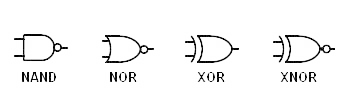
\includegraphics[trim={.5cm 0 4cm 0},clip,width=\textwidth]{gates.png}
  \end{marginfigure}

De `not and'-operator (NAND), ook wel \textbf{Sheffer Stroke} genaamd, wordt in de logica geschreven als $\uparrow$ en werkt hetzelfde als de NAND-gate (zie ook de waarheidstabel hieronder). Ze kan ook worden uitgedrukt als $\neg(p\land q)$.

De `not or'-operator (NOR) is haar directe tegenhanger (zie ook de waarheidstabel), en is in de logica ook wel bekend als \textbf{Peirce Arrow} of \textbf{Quine Dagger}. Ze wordt geschreven als $\downarrow$ en werkt vergelijkbaar als de NOR-gate. Ze kan ook worden uitgedrukt als $\neg(p\lor q)$ (zie ook de waarheidstabellen).

Een markant detail is dat zowel de Sheffer Stroke als de Quine Dagger \textit{op zichzelf} voldoende is om alle andere connectieven af te kunnen leiden (zie sectie \ref{sec:volledig}).
$$\begin{array}{ccc}
p&q&p\oplus q\\
\hline
0&0&0\\
0&1&1\\
1&0&1\\
1&1&0
\end{array}\quad
\begin{array}{ccc}
p&q&p\uparrow q\\
\hline
0&0&1\\
0&1&1\\
1&0&1\\
1&1&0
\end{array}\quad
\begin{array}{ccc}
p&q&p\downarrow q\\
\hline
0&0&1\\
0&1&0\\
1&0&0\\
1&1&0
\end{array}
$$
\end{aside}

\subsection{Opgaven}
\begin{exercise}[Waarheidstabellen]\mbox{}\\
Construeer de waarheidstabellen van de volgende samengestelde proposities:
\begin{enumerate}[label=\textit{\alph*.}]
\item $(p\land q)\land((\neg q)\lor r)$
\item $p\rightarrow(q\lor r)$
\item $\neg((\neg p)\lor\neg((\neg q)\lor\neg p))$
\item $p\leftrightarrow(q\leftrightarrow r)$
\item $p\leftrightarrow(q\leftrightarrow p)$
\end{enumerate}
\end{exercise}

\section{Metaredeneren}
%\todo[inline,color=hured!40]{Logisch gevolg, onderscheid syntax/semantiek, equivalentie, meta-beweringen}
Logica analyseert niet alleen bestaande vormen van redeneren, maar probeert ook de eigenschappen van die systemen te analyseren. De propositielogica is daarvan een uitstekend voorbeeld; het kan gebruikt worden om stelselmatige wetmatigheden te bestuderen.

Logici zijn al eeuwen ge\"interesseerd in `speciale' formules, bijvoorbeeld $p\lor\neg p$ en $p\land\neg p$. De eerste is immers nooit onwaar, de tweede is nooit waar. Deze eigenschappen van formules kunnen we afleiden uit de waarheidstabellen van de formule, en we kunnen uitzoeken welke eigenschappen van de waarheidstabellen van de formule in kwestie hiervoor verantwoordelijk zijn.

Een andere wetmatigheid heeft te maken met redeneringen. Waarom vinden we dat een redenering van de vorm `uit $p\lor\neg q$ en $q$ kan men $p$ afleiden' correct (geldig), en welke eigenschappen van de waarheidstabellen van de formules in kwestie zijn hiervoor verantwoordelijk.

Door op zo'n wiskundige manier te denken kunnen we dus precies defini\"eren wat geldigheid is, maar kunnen we hiermee ook allerlei mooie patronen zien in geldig redeneren die anders onzichtbaar zouden blijven. Voorbeelden die we zullen zien zijn de dualiteit van conjunctie en disjunctie in de aanwezigheid van negatie, en het systematisch aan elkaar schakelen van implicaties.

Deze vorm van redeneren over het redenatie-systeem (oftewel eigenschappen proberen te ontlenen aan de wetmatigheden van de logica) wordt ook wel meta-redeneren genoemd (redeneren over het redeneren). Hoewel het soms erg verwarrend kan zijn (beide zijn immers redenaties) is het uiterst belangrijk om uitspraken op het meta-niveau te onderscheiden van uitspraken op het redenatie-niveau (vergelijk met metataal vs. objecttaal in sectie \ref{sec:metataal}). Dit onderscheid vindt zijn grondslag in het verschil tussen de syntax en de semantiek van de propositielogica. Uitspraken over geldigheid, het gevolg van redeneringen, etc., hebben allen betrekking op de semantiek (betekenis) van de logica, en dienen derhalve dus te worden uitgedrukt in symbolen die anders zijn de de symbolen die worden gebruikt om de argumenten te noteren (de syntax). 

\subsection{Tautologie\"en}
Sommige proposities zijn steeds waar, andere zijn soms waar en soms onwaar, afhankelijk van de situatie waarop ze betrekking hebben. Zo is \enquote{de brug is open} waar als de brug open is, en anders is deze uitspraak onwaar. Wanneer men in een computerprogramma twee variabelen $x$ en $y$ heeft, dan is de als test te gebruiken propositie \enquote{$x=y$} waar als $x$ en $y$ dezelfde waarde hebben, en anders onwaar. De propositie \enquote{$x=x$} is echter altijd waar.

Wat ons vooral interesseert zijn samengestelde proposities en hoe men aantoont dat een propositie steeds waar is. Bij een uit een klein aantal proposities $p, q, r,\ldots$ samengestelde propositie $A$ kan men gemakkelijk controleren of $A$ steeds waar is door de waarheidstabel van $A$ op te stellen en te kijken of de waarheidswaarde van $A$ steeds $1$ is. De elementaire bouwstenen $p, q, r,\ldots$ heten wel \textit{atomen} of \textit{atomaire proposities}. Omdat elk atoom twee waarheidswaarden kan hebben, bestaat de waarheidstabel voor een proposities opgebouwd uit $n$ verschillende atomen uit $2^n$ regels. Voor een $n=3$ of $n=4$ is dat nog best te doen, maar als $n$ minstens $10$ is, zijn er toch wel minstens duizend regels nodig, en komt de vraag op of het niet met minder werk kan.

We zullen nu een manier aangeven om te manipuleren met samengestelde proposities, het vervangen van een propositie door een andere propositie met dezelfde betekenis. Met dergelijke manipulaties is het opstellen en nalopen van waarheidstabellen vaak te vermijden.

Twee proposities $A$ en $B$, beide opgebouwd uit $p, q, r,\ldots$, hebben dezelfde betekenis precies dan als $A\leftrightarrow B$ steeds waar is. Dit is hetzelfde als zeggen dat de waarheidstabellen van $A$ en $B$ aan elkaar gelijk zijn.

\begin{definition}[Tautologie]\mbox{}\\
Een \textit{tautologie} is een steeds ware propositie, oftewel voor elke keuze van waarheidswaarden voor de erin voorkomende atomen is de waarheidswaarde van de propositie $1$.
\end{definition}
%
Een propositie is dus een tautologie als hij dezelfde waarheidstabel heeft als $\top$.

Hieronder volgt een lijstje van belangrijke tautologie\"en, zodat we die niet telkens weer opnieuw hoeven te bewijzen. De in de lijst voorkomende letters zijn atomen. Hiervoor mag men willekeurige concrete proposities invullen (ook samengestelde proposities) onder de voorwaarde dat voor dezelfde propositieletter ook steeds dezelfde (samengestelde) propositie wordt ingevuld.

\begin{theorem}\mbox{}\\
Alle proposities in de volgende lijst zijn tautologie\"en:
\begin{enumerate}
\item $p\lor\neg p$
\item $\neg(p\land\neg p)$
\item $p\rightarrow(q\rightarrow p)$
\item $\neg p\rightarrow(p\rightarrow q)$
\item $(p\land\neg p)\rightarrow q$
\item $(p\leftrightarrow q)\rightarrow(p\rightarrow q)$
\item $((p\rightarrow q)\land(q\rightarrow r))\rightarrow(p\rightarrow r)$
\item $(p\rightarrow q)\lor(q\rightarrow p)$
\item $(p\rightarrow q)\rightarrow((q\rightarrow r)\rightarrow(p\rightarrow r))$
\item $((p\rightarrow q)\land(r\rightarrow s))\rightarrow((p\land r)\rightarrow(q\land s))$
\item $((p\rightarrow q)\lor(r\rightarrow s))\rightarrow((p\land r)\rightarrow(q\lor s))$
\item $((p\leftrightarrow q)\land(q\leftrightarrow r))\rightarrow(p\leftrightarrow r)$
\item $\top$
\item $\neg\bot$
\end{enumerate}
\end{theorem}

Het lijkt een lange lijst, maar de regels 1 t/m 6 liggen nogal voor het oprapen. Regel 7 drukt uit dat implicatie \textit{transitief} is. Hopelijk geven regels 8 en 11 de lezer het gevoel dat het niet allemaal zo vanzelfsprekend is.

Een stelling is pas echt een stelling als er ook een bewijs bij is; in dit geval betekent dat dat we voor elke regel moeten bewijzen dat de genoemde propositie een tautologie is. Dat kunnen we met waarheidstabellen doen: als we systematisch alle mogelijke combinaties van waarheidswaarden voor $p, q$ en $r$ afgaan en zien dat de waarheidswaarde van de propositie in alle gevallen $1$ is, hebben we bewezen dat het een tautologie is. Dit doen we hier alleen voor regel 7; voor de overige regels gaat het op soortgelijke wijze en laten we het aan de lezer over. Voor regel 7 moeten we laten zien dat $((p\rightarrow q)\land(q\rightarrow r))\rightarrow(p\rightarrow r)$ een tautologie is, en daarvoor moeten we eerst de waarheidswaarden van $p\rightarrow q$, van $q\rightarrow r$, van $(p\rightarrow q)\wedge(q\rightarrow r)$ en van $p\rightarrow r$ bepalen. Dat zouden we afzonderlijk kunnen doen door hier aparte waarheidstabellen van te maken, maar het kan ook in \'e\'en keer met een grote waarheidstabel, waarin we onder de pijl van $p\rightarrow q$ de waarheidswaarde van $p\rightarrow q$ noteren, vervolgens onder de pijl van $q\rightarrow r$ de waarheidswaarde van $q\rightarrow r$, enzovoorts:
\begin{proof} $((p\rightarrow q)\land(q\rightarrow r))\rightarrow(p\rightarrow r)$ is een tautologie:
\begin{center}
\begin{tikzpicture}[node distance=1mm and 0mm,baseline]
\matrix (M1) [matrix of nodes, column sep=1em]
{
  $p$ & $q$ & $r$ & $((p\rightarrow q)$ & $\land$ & $(q\rightarrow r))$ & $\rightarrow\ $ & $(p\rightarrow r)$ \\
  0 & 0 & 0 & 1 & 1 & 1 & 1 & 1 \\
  0 & 0 & 1 & 1 & 1 & 1 & 1 & 1\\
  0 & 1 & 0 & 1 & 0 & 0 & 1 & 1 \\
  0 & 1 & 1 & 1 & 1 & 1 & 1 & 1 \\
  1 & 0 & 0 & 0 & 0 & 1 & 1 & 0 \\
  1 & 0 & 1 & 0 & 0 & 1 & 1 & 1 \\
  1 & 1 & 0 & 1 & 0 & 0 & 1 & 0 \\
  1 & 1 & 1 & 1 & 1 & 1 & 1 & 1 \\
};
\draw (M1-1-1.south west) -- (M1-1-8.south east);
\draw (M1-1-1.north west) -- (M1-9-1.south west) -- (M1-9-8.south east -| M1-1-8.east) -- (M1-1-8.north east);
\draw[hublue, ultra thick] (M1-1-7.north west) rectangle (M1-9-7.south east);
\end{tikzpicture}
\end{center}
\end{proof}
Inderdaad zien we in de rood omrande kolom alleen maar enen staan, waarmee bewezen is dat de hele propositie een tautologie is.

In principe maakt de volgorde van de mogelijke combinaties van waarheidswaarden niet uit, als alle mogelijke combinaties maar opgesomd worden. Hier is de systematiek gevolgd waarbij het laatste atoom ($r$) afwisselend 0 en 1 is ingevuld, bij het voorlaatste ($q$) afwisselend twee nullen en twee enen, en daar weer voor (bij $p$) eerst vier nullen en dan vier enen. Dit breidt op een voor de hand liggende manier uit naar elk willekeurig aantal atomen: bij $n$ atomen staan er in de eerste $n$ kolommen de getallen van 0 tot en met $2^n-1$ in \textit{binaire notatie}.

Twee hieraan verwante begrippen die nog ge\"introduceerd dienen te worden zijn \textit{contradictie} en \textit{contingentie}.
\begin{definition}[Contradictie]\mbox{}\\
Een \textit{contradictie} is een steeds onware propositie, oftewel voor elke keuze van waarheidswaarden voor de erin voorkomende atomen is de waarheidswaarde van de propositie $0$.
\end{definition}
Een propositie is dus een contradictie als hij dezelfde waarheidstabel heeft als $\bot$.
\begin{definition}[Contingentie]\mbox{}\\
Een \textit{contingentie} is een propositie die soms waar en soms onwaar is, oftewel voor enkele keuzes van waarheidswaarden voor de erin voorkomende atomen (maar voor tenminste \'e\'en) is de waarheidswaarde van de propositie $1$ \'en voor enkele keuzes van waarheidswaarden voor de erin voorkomende atomen (maar voor tenminste \'e\'en) is de waarheidswaarde van de propositie $0$.
\end{definition}
Een propositie is dus een contingentie als hij noch een tautologie, noch een contradictie is.

\subsection{Equivalenties}\label{sec:equiv}
Hoewel het maken van een waarheidstabel een eenvoudige (doch bewerkelijke) exercitie is, kan het in het geval dat een samengestelde propositie veel atomen bevat toch gauw uit de klauw lopen. Zoals eerder genoemd is voor het maken van een waarheidstabel van een propositie met $n$ verschillende atomaire proposities een waarheidstabel benodigd met $2^n$ rijen.

Gelukkig zijn er effectievere methoden om te bepalen of de waarheidstabellen van twee proposities gelijk aan elkaar zijn. Hiervoor introduceren wij het begrip \textit{equivalentie}.
%
\begin{definition}[Equivalentie]\mbox{}\\
Twee proposities $A$ en $B$ heten \textit{gelijkwaardig} of \textit{equivalent} als $A\leftrightarrow B$ een tautologie is, oftewel voor elke keuze van waarheidswaarden voor de erin voorkomende atomen is de waarheidswaarde van $A$ gelijk aan die van $B$.

\noindent
We schrijven dan wel $A\equiv B$, of ook wel $A\Leftrightarrow B$\footnote{Bemerk hier ook weer het onderscheid tussen \textit{syntax} en \textit{semantiek}: $A\leftrightarrow B$ drukt syntactisch uit dat $A$ en $B$ equivalent zijn, zoals gedefinieerd voor het geldende connectief (zie definitie \ref{def:bi}). $A\equiv B$ of $A\Leftrightarrow B$ drukken \textit{semantisch} uit dat de \textit{waarde van $A$} hetzelfde is als de \textit{waarde van $B$}.}.
\end{definition}

In de volgende tabel presenteren wij een aantal veel voorkomende en gebruikte equivalenties. Het nut van zo'n tabel is dat deze je basispatronen biedt die je kan gebruiken om complexe samengestelde proposities te vereenvoudigen.

\begin{theorem}
De proposities in de volgende lijst zijn op eenzelfde regel gelijkwaardig aan elkaar\\
$\begin{array}{*7l}
1. & p & \neg(\neg p) & p\land p\quad{} & p\lor p & p\lor\bot\quad{} & p\land\top \\
2. & p\lor q & q\lor p \\
3. & p\land q & q\land p\\
4. & p\leftrightarrow q & q\leftrightarrow p & \multicolumn{2}{l}{(p\rightarrow q)\land(q\rightarrow p)} & \multicolumn{2}{l}{(p\land q)\lor(\neg p \land\neg q)} \\
5. & (p\lor q)\lor r & p\lor(q\lor r) \\
6. & (p\land q)\land r & p\land(q\land r) \\
7. & p\rightarrow q & \neg p\lor q & \neg q \rightarrow\neg p \\
8. & \neg(p\rightarrow q) & p\land\neg q \\
9. & \neg(p\lor q) & \neg p\land\neg q \\
10. & \neg(p\land q) & \neg p \lor\neg q \\
11. & (p\lor q)\land r & \multicolumn{2}{l}{(p\land r)\lor(q\land r)} \\
12. & (p\land q)\lor r & \multicolumn{2}{l}{(p\lor r)\land(q\lor r)} \\
13. & (p\lor q)\rightarrow r & \multicolumn{2}{l}{(p\rightarrow r)\land(q\rightarrow r)} \\
14. & p\rightarrow(q\land r) & \multicolumn{2}{l}{(p\rightarrow q)\land (p\rightarrow r)} \\
15. & p\rightarrow(q\rightarrow r) & (p\land q)\rightarrow r \\
16. & p\lor\neg p & p\lor\top & \top \\
17. & p\land\neg p & p\land\bot & \bot 
\end{array}$\label{th:equiv}
\end{theorem}

Regels 2, 3 en 4 (eerste deel) geven aan dat de operatoren $\lor$, $\land$, en $\leftrightarrow$ \textit{commutatief} zijn. Regels 5 en 6 geven aan dat de operatoren $\lor$ en $\land$ \textit{associatief} zijn. Regel 7 geeft eigenlijk de definitie van de implicatie en tevens de contrapositie. Regels 8, 9 en 10 laten zien hoe we met ontkenningen moeten omgaan. Regels 9 en 10 staan bekend als de \textit{wetten van De Morgan}.

Regels 11 en 12 beschrijven dat $\lor$ en $\land$ \textit{distributief} zijn, preciezer: regel 11 zegt dat $\land$ \textit{distribueert over} $\lor$, en regel 12 zegt dat $\lor$ distribueert over $\land$. Regel 16 en 17 geven nog enkele voordehandliggende verbanden met $\top$ en $\bot$.

Van deze lijst is het handig om in ieder geval regels 1 t/m 12 en 16, 17 te kennen en altijd paraat te hebben.

Ook deze stelling kan zonder enig probleem worden bewezen door voor de onderhavige proposities de waarheidstabellen op te stellen en te controleren dat de zaak klopt: steeds moet je laten zien dat proposities op dezelfde regel precies gelijke kolommen geven in de waarheidstabel. Nadat de equivalenties uit de stelling zijn bewezen, echter, kan je deze toepassen om complexe samenstellingen te vereenvoudigen.

Voor het toepassen van Stelling \ref{th:equiv} zijn de volgende opmerkingen van groot belang:
\begin{itemize}
\item Voor $p, q, r,\ldots$ mogen steeds willekeurige proposities worden ingevuld;
\item De regels zijn niet alleen van toepassing op de hele uitdrukking, maar ook op delen daarvan. Zo mogen we uit $A\equiv B$ concluderen: $\neg A\equiv\neg B$, $p\lor A\equiv p\lor B$, $A\lor p\equiv B\lor p$, $p\land  A\equiv p\land B$, et cetera.
\end{itemize}

Het op deze wijze toepassen van Stelling \ref{th:equiv} en andere spelregels van dit hoofdstuk wordt soms ook wel \textit{propositierekening} of \textit{equivalentierekenen} genoemd.

Een dergelijke methode kan ook worden gebruikt om andere regels van Stelling \ref{th:equiv} te bewijzen. Als voorbeeld laten we zien hoe regel 10 van Stelling \ref{th:equiv} volgt uit andere regels door proposities te vervangen door gelijkwaardige proposities\footnote{Voor de hier gebruikte regels 1, 7 en 9 dient natuurlijk ook een bewijs te worden gegeven, bijv. door middel van een waarheidstabel. Dit laten wij hier aan de lezer over.}. Een dergelijk bewijs heet een \textit{equitioneel bewijs}.
\begin{proof}\mbox{}\\
$\begin{array}{llll}
\neg(p\rightarrow q) & \equiv & \neg(\neg p\lor q) & \text{(regel 7)}\\
& \equiv & \neg(\neg p)\land\neg q & \text{(regel 9)} \\
& \equiv & p\land\neg q & \text{(regel 1)}
\end{array}$\\
\end{proof}

Op deze manier kunnen we ook nieuwe gelijkwaardigheden worden afgeleid, bijvoorbeeld\\
$\begin{array}{llll}
p\land(q\lor r) & \equiv & (q\lor r)\land p & \text{(regel 3)} \\
& \equiv & (q\land p)\lor(r\land p) & \text{(regel 11)} \\
& \equiv & (p\land q)\lor(r\land p) & \text{(regel 3)} \\
& \equiv & (p\land q)\lor(p\land r) & \text{(regel 3)}
\end{array}$

Door herhaaldelijk toepassen van de regels 2 en 5 van Stelling \ref{th:equiv} kan men laten zien dat in $p\lor q\lor\ldots\lor r$ de haakjes willekeurig geplaatst mogen worden, en dat de volgorde er niet toe doet. Daarom laten we in samenstellingen met alleen het connectief $\lor$ vaak de haakjes weg.

Eenzelfde opmerking geldt voor $p\land q\land\ldots\land r$, hetgeen volgt door herhaaldelijk toepassen van regels 3 en 6.

\subsection{Logisch Gevolg}
Met de hier ontwikkelde begrippen zijn we nu in staat om een precieze logische definitie te geven van wat we intu\"itief een correcte redenering noemen. Welke eigenschap van de waarheidstabellen van de betrokken formules is hiervoor verantwoordelijk?

Om dit te achterhalen, beschouwen we een eenvoudige redenering: uit `Jan is een goede schaker en Karin een goede dammer' kan worden geconcludeerd: `Jan is een goede schaker'. Het uitgangspunt is `Jan is een goede schaker en Karin is een goede dammer' en de conclusie is `Jan is een goede schaker'. Hier is geen speld tussen te krijgen: de redenering is correct. Zij nu $p =$ `Jan is een goede schaker' en $q =$ `Karin is een goede dammer'. We maken vervolgens de waarheidstabellen van het uitgangspunt (premisse) $(p\land q)$ en de conclusie $p$:\\
\begin{tikzpicture}[node distance=1mm and 0mm,baseline]
\matrix (M) [matrix of nodes, column sep=1em]
{
  $p$ & $q$ & $p\land q$ & $p$ \\
  0 & 0 & 0 & 0 \\
  0 & 1 & 0 & 0 \\
  1 & 0 & 0 & 1 \\
  1 & 1 & 1 & 1 \\
};
\draw (M-1-1.south west) -- (M-1-4.south east);
\draw (M-1-1.north west) -- (M-5-1.south west) -- (M-5-4.south east -| M-1-4.east) -- (M-1-4.north east);
\draw[hublue,ultra thick] (M-1-3.north west) rectangle (M-5-3.south east -| M-1-3.east);
\draw[hublue,ultra thick] (M-1-4.north west) rectangle (M-5-4.south east);
\end{tikzpicture}

Vergelijken we de aangegeven kolommen, dan valt op dat het uitgangspunt en de conclusie niet altijd tegelijk waar zijn, en niet dezelfde waarheidswaarde hoeven te hebben, maar dat, en dit is essentieel:
\begin{quote}
als het uitgangspunt waar is, dan is ook de conclusie waar.
\end{quote}
We spreken van \textit{logisch gevolg} of van `geldige gevolgtrekking'.

\begin{definition}[Logisch gevolg]\label{def:gevolg}
De formule $\psi$ is een logisch gevolg van $\varphi_1,\ldots,\varphi_n$ als elke waardering die alle $\varphi_1,\ldots,\varphi_n$ waar maakt, ook $\psi$ waar maakt.\\
We schrijven hiervoor $\varphi_1,\ldots,\varphi_n\Rightarrow\psi$ of $\varphi_1,\ldots,\varphi_n\therefore\psi$.
\end{definition}

\begin{example}
De redenering in het vorige voorbeeld kunnen we weergeven als $p\land q\therefore p$, dat wil zeggen: $p$ is een logisch gevolg van $p\land q$. Immers, er was blijkens de tabel maar \'e\'en waardering die $p\land q$ waar maakte (de laatste regel), en die maakt inderdaad de conclusie $p$ ook waar.\\
In dit voorbeeld is $n=1$ en $\varphi_1$ de formule $p\land q$.
\end{example}

\begin{example}
Gegeven is de volgende redenering:
\begin{quote}
`De afstandsbediening is kapot of de tv werkt niet goed. Maar de tv werkt wel goed. Dus de afstandsbediening is kapot.'
\end{quote}
We kiezen nu $p=$ `De afstandsbediening is kapot' en $q=$ `De tv werkt goed'. We gaan nu kijken of $p$ een logisch gevolg is van $p\lor\neg q$ en $q$ samen.\\
\begin{tikzpicture}
\matrix (M) [matrix of nodes, column sep=1em] {
    $p$ & $q$ & $\neg q$ & $p\lor\neg q$ & $q$ & $p$ \\
    0 & 0 & 1 & 1 & 0 & 0 \\
    0 & 1 & 0 & 0 & 1 & 0 \\
    1 & 0 & 1 & 1 & 0 & 1 \\
    1 & 1 & 0 & 1 & 1 & 1 \\
};
\draw (M-1-1.south west) -- (M-1-6.south east);
\draw (M-1-1.north west) -- (M-5-1.south west) -- (M-5-6.south east -| M-1-6.east) -- (M-1-6.north east);
\draw[hublue,ultra thick] (M-5-4.north west) rectangle (M-5-4.south east);
\draw[hublue,ultra thick] (M-5-5.north west) rectangle (M-5-5.south east);
\end{tikzpicture}

\noindent
Uit de tabel blijkt dat de beide uitgangspunten alleen tegelijk waar zijn (omrandde enen) als $p$ en $q$ waar zijn (laatste regel). Met andere woorden: we hoeven slechts naar de laatste rij waarheidswaarden te kijken, en daar is de conclusie ook waar. Kortom: $p\lor\neg q,q\therefore p$. In dit voorbeeld is $n=2$, $\varphi_1$ de formule $p\lor\neg q$ en $\varphi_2$ de formule $q$.
\end{example}

Merk op dat in de definitie van geldig gevolg staat: \textit{elke} waardering die de uitgangspunten waar maakt, moet de conclusie waar zijn. Het is niet voldoende dat er \textit{een} waardering bestaat die zowel uitgangspunten als conclusie waar maakt.

\begin{example}\label{ex:no:gevolg}
Uit `Er komen meer wegen in Nederland precies dan als Nederland geasfalteerd raakt' is niet correct te concluderen dat er meer wegen in Nederland komen. Formeel $p\leftrightarrow q\not\therefore p$, dat wil zeggen, $p$ is geen logisch gevolg van $p\leftrightarrow q$. Er is \textit{een} waardering die het uitgangspunten en de conclusie waarmaakt, namelijk de waardering die $p$ en $q$ allebei waarmaakt. Maar er is ook een waardering die $p\leftrightarrow q$ waarmaakt, maar niet de conclusie, namelijk de waardering die $p$ en $q$ allebei onwaar maakt.\\
\begin{tikzpicture}
\matrix (M) [matrix of nodes, column sep=1em] {
    $p$ & $q$ & $p \leftrightarrow q$ & $q$  \\
    0 & 0 & 1 & 0 \\
    0 & 1 & 0 & 1 \\
    1 & 0 & 0 & 0 \\
    1 & 1 & 1 & 1 \\
};
\draw (M-1-1.south west) -- (M-1-4.south east);
\draw (M-1-1.north west) -- (M-5-1.south west) -- (M-5-4.south east -| M-1-4.east) -- (M-1-4.north east);
\draw[hublue,ultra thick] (M-5-3.north west) rectangle (M-5-3.south east);
\draw[hublue,ultra thick] (M-5-4.north west) rectangle (M-5-4.south east);
\draw[hublue,ultra thick] (M-2-3.north west) rectangle (M-2-3.south east);
\draw[hublue,ultra thick] (M-2-4.north west) rectangle (M-2-4.south east);
\node at (2.5,-.85) {\color{green!70!black}{\usym{2714}}};
\node at (2.5,.35) {\color{red}{\large\usym{2718}}};
\end{tikzpicture}
\end{example}

Een aantal bekende vormen van gevolgtrekkingen zijn:\\
\begin{tabular}{|p{4cm}p{6cm}|}
\hline
\textit{naam}&\textit{vorm van de gevolgtrekking}\\
&\\
uitgesloten derden&$\neg\neg\varphi\therefore\varphi$\\
modus ponens&$\varphi,\varphi\rightarrow\psi\therefore\psi$\\
contrapositie&$\varphi\rightarrow\psi\therefore\neg\psi\rightarrow\neg\varphi$\\
hypothetisch syllogisme&$\varphi\rightarrow\psi,\psi\rightarrow\chi\therefore\varphi\rightarrow\chi$\\
\hline
\end{tabular}\label{tab:gevolg}\vspace{2mm}

Deze regels worden (vaak stilzwijgend) gebruikt bij wiskundige bewijzen.

\begin{aside}[Symbool voor logisch gevolg]\mbox{}\\
Logisch gevolg wordt, in verschillende bronnen, uitgedrukt door middel van verschillende symbolen: $\vdash$, $\vDash$ of $\therefore$.

Het symbool $\vdash$ werd voor het eerst gebruikt door Gottlob Frege in zijn \textit{Begriffschrifft} (\citeyear{frege:begriffschrift}) om \textit{afleidbaarheid} aan te duiden. Het wordt klassiek gelezen als \enquote{maakt waar}, \enquote{bewijst dat}, \enquote{vervult} of \enquote{brengt met zich mee}. Het symbool zelf wordt ook wel \textbf{turnstile} (draaihekje) genoemd, omdat het er enigszins op lijkt (van boven gezien). Het wordt soms ook \textbf{tee} genoemd. Het is het universele symbool voor \textit{beweringen}, waarbij $\vdash A$ gelezen wordt als \textit{ik weet dat $A$ waar is} (of \textit{uit niets is $A$ af te leiden}). Soortgelijk leest men afhankelijke beweringen als $P\vdash Q$ als \textit{vanuit $P$ weet ik dat $Q$} (ofwel, \textit{gegeven $P$ weet ik dat $Q$}, of \textit{gegeven $P$ kan ik $Q$ afleiden}).

De semantische tegenhanger is de dubbele turnstile $\vDash$, welke wordt gebruikt om semantisch gevolg aan te duiden; als alles aan de linkerzijde van het symbool waar is, dan moet de bewering aan de rechterzijde ook waar zijn, bijv. $\Gamma\vDash A$. Merk op dat dit erg verwant is aan de enkele turnstile, die syntactisch gevolg aanduidt (uit de syntactische beweringen links zijn de beweringen rechts af te leiden). $\vDash$ geeft hiermee \textit{vervulbaarheid} aan, terwijl $\vdash$ \textit{afleidbaarheid} aanduidt... maar we begrijpen dat dit verschil voor de meesten erg minimaal is en lastig te onderscheiden.

Het dus-teken $\therefore$ tenslotte, is een logisch en wiskundig symbool gebruikt in bewijzen om een gevolg (conclusie) aan te duiden. Je zou het in een redenering kunnen vervangen door het woordje `dus'. Omdat het een semantische betekenis heeft (je koppelt de betekenis van de beweringen aan elkaar om tot een conclusie te komen), is ze verwant aan $\vDash$. Merk overigens op dat ze de tegenhanger is van het \textit{omdat-teken} ($\because$).
\end{aside}

\subsection{Opgaven}
\begin{exercise}\mbox{}\\
Bewijs met behulp van waarheidstabellen dat
\begin{enumerate}[label=\textit{\alph*.}]
\item $((p\rightarrow q)\lor(r\rightarrow s))\rightarrow((p\land r)\rightarrow(q\lor s))$ een tautologie is.
\item $((p\rightarrow q)\land(q\rightarrow r))\rightarrow(p\rightarrow r)$ een tautologie is.
\item $\neg(p\rightarrow\neg q)$ en $p\land q$ gelijkwaardig zijn.
\end{enumerate}
\end{exercise}

\begin{exercise}\mbox{}\\
Bewijs door gebruik te maken van één van de gelijkwaardige proposities uit Stelling \ref{th:equiv}, dat de onderstaande paren van proposities gelijkwaardig aan elkaar zijn. De eerste is voorgedaan.
\begin{enumerate}[label=\textit{\alph*.}]
% a:
\item $\neg ((d\leftrightarrow e)\vee d)$ en $\neg (d\leftrightarrow e) \wedge \neg d$ \\
antwoord:
\begin{align}
\neg ((d\leftrightarrow e)\vee d) &\equiv \neg (d\leftrightarrow e)\wedge \neg d  \tag{St-\ref{th:equiv}: 9}
\end{align}
%b:
\item $(e\land h) \leftrightarrow b$ en $((e\land h) \land b) \lor (\neg (e\land h)\land \neg b)$
%c:
\item $(a\lor (b\rightarrow a)) \rightarrow z$ en $(a\rightarrow z)\land ((b\rightarrow a) \rightarrow z)$
%d:
\item $(p\land \neg e)\lor (\neg e \rightarrow q)$ en $(\neg e\rightarrow q)\lor (p\land \neg e)$
%e:
\item $a \leftrightarrow (b\rightarrow a)$ en $a \leftrightarrow (\neg a\rightarrow \neg b)$ 
%f:
\item $(h \land (f\lor z))\rightarrow q$ en $h\rightarrow ((f\lor z) \rightarrow q)$  
%g:
\item $\neg (p\leftrightarrow q)\lor \neg z$ en $\neg ((p\leftrightarrow q) \land z)$  
%h:
\item $q \rightarrow \neg \neg (h \leftrightarrow z) $ en $q \rightarrow (h \leftrightarrow z)$ 
\end{enumerate}
\end{exercise}

\begin{exercise}\mbox{}\\
Bewijs door gebruik te maken van twee of meer van de gelijkwaardige proposities uit Stelling \ref{th:equiv}, dat de onderstaande paren van proposities gelijkwaardig aan elkaar zijn. De eerste is voorgedaan.
\begin{enumerate}[label=\textit{\alph*.}]
% a:
\item $(\neg b\land a)\lor \neg (a\lor \neg b)$ en $a\leftrightarrow \neg b$\\
antwoord:
\begin{align}
(\neg b\wedge a)\vee \neg (a\vee \neg b) &\equiv (\neg b\wedge a)\vee (\neg a \wedge \neg \neg b)  \tag{St-\ref{th:equiv}: 9} \\
&\equiv (a\wedge \neg b)\vee (\neg a \wedge \neg \neg b)  \tag{St-\ref{th:equiv}: 3} \\
&\equiv a\leftrightarrow \neg b\tag{St-\ref{th:equiv}: 4}
\end{align}
% b:
\item $z\land ((q\rightarrow e) \lor (q\rightarrow e))$ en $(q \rightarrow e) \land z$
% c:
\item $\neg (m\land h)$ en $m \rightarrow \neg h$
% d:
\item $(n \lor r)\rightarrow (p \land r)$ en $((n \lor r)\rightarrow p) \land (\neg r \rightarrow \neg (n \lor r))$
% e:
\item $\neg (\neg a \rightarrow z)$ en $\neg a \land \neg (\neg z\rightarrow z)$
% f:
\item $\neg(p\rightarrow q) \lor (\neg (q \rightarrow p) \lor r)$ en $\neg (p\leftrightarrow q) \lor r$
% g:
\item $(z\lor k)\rightarrow m$ en $(\neg z \lor m) \land (\neg k \lor m)$
% h:
\item $c \land (h\leftrightarrow d)$ en $\neg (c \rightarrow \neg (d \leftrightarrow h))$  

\end{enumerate}
\end{exercise}

\begin{exercise}\mbox{}\\
Bewijs dat regels 13, 14 en 15 van Stelling \ref{th:equiv} inderdaad gelijkwaardige proposities aangeven.
\end{exercise}

\begin{exercise}\mbox{}\\
Bewijs door uitsluitend te vervangen door gelijkwaardige proposities uit Stelling \ref{th:equiv}, dat
\begin{enumerate}[label=\textit{\alph*.}]
\item $a\leftrightarrow b$ en $\neg a \leftrightarrow \neg b$ gelijkwaardig zijn.
\item $(\neg a\land\neg b)\rightarrow c$ en $\neg a\rightarrow(b\lor c)$ gelijkwaardig zijn.
\end{enumerate}
\end{exercise}

\begin{exercise}\mbox{}\\
Oom Henk heeft altijd de grootste verhalen. Zijn jonge neefjes en nichtjes zijn meer van \enquote{goed verhaal, lekker kort}. Nu wil oom Henk graag wat propositielogica aan zijn neefjes en nichtjes laten zien, maar ook bij zijn propositielogica heeft hij last van zijn breedsprakigheid. Help oom Henk met hip zijn en versimpel de onderstaande propositie zo veel mogelijk  Er is er al één voorgedaan. 
\begin{enumerate}[label=\textit{\alph*.}]
% a:
\item $\neg ((a\land b) \lor \neg(\neg a \rightarrow b))$\\
antwoord:
\begin{align}
\neg ((a\wedge b)\vee \neg (\neg a\rightarrow b)) &\equiv \neg (a\wedge b) \wedge \neg \neg (\neg a\rightarrow b)  \tag{St-\ref{th:equiv}: 9} \\
&\equiv \neg (a\wedge b) \wedge (\neg a\rightarrow b)   \tag{St-\ref{th:equiv}: 1} \\
&\equiv (\neg a \vee \neg b) \wedge (\neg a\rightarrow b) \tag{St-\ref{th:equiv}: 10} \\
&\equiv (\neg a \vee \neg b) \wedge (\neg a\rightarrow \neg \neg b) \tag{St-\ref{th:equiv}: 1} \\
&\equiv (\neg a \vee \neg b) \wedge (\neg b \rightarrow a) \tag{St-\ref{th:equiv}: 7} \\
&\equiv (a \rightarrow \neg b) \wedge (\neg b \rightarrow a) \tag{St-\ref{th:equiv}: 7} \\
&\equiv a \leftrightarrow \neg b \tag{St-\ref{th:equiv}: 4}
\end{align}
% b:
\item $\neg (p \rightarrow \neg (q \rightarrow q))$
% c:
\item $\neg((\neg p\rightarrow q)\rightarrow ((p\rightarrow\neg r)\wedge(r\rightarrow q)))$
\end{enumerate}
\end{exercise}

\begin{exercise}\mbox{}\\
Bepaal voor alle volgende stellingen of het altijd, soms of nooit een logisch gevolg is (maak zo nodig een waarheidstabel om te checken):
\begin{enumerate}[label=\textit{\alph*.}]
\item $\varphi\vdash\psi$ als $\varphi$ en $\psi$ beiden een tautologie zijn;
\item $\varphi\vdash\psi$ als $\varphi$ een tautologie is en $\psi$ een contradictie;
\item $\varphi\vdash\psi$ als $\varphi$ een tautologie is en $\psi$ een contingentie;
\item $\varphi\vdash\psi$ als $\varphi$ een contradictie is en $\psi$ een tautologie;
\item $\varphi\vdash\psi$ als $\varphi$ een contradictie is en $\psi$ een contradictie;
\item $\varphi\vdash\psi$ als $\varphi$ een contradictie is en $\psi$ een contingentie;
\item $\varphi\vdash\psi$ als $\varphi$ een contingentie is en $\psi$ een tautologie;
\item $\varphi\vdash\psi$ als $\varphi$ een contingentie is en $\psi$ een contradictie;
\item $\varphi\vdash\psi$ als $\varphi$ een contingentie is en $\psi$ een contingentie;
\end{enumerate}
\end{exercise}

\section{Functionele compleetheid}\label{sec:volledig}
%\begin{remark}
%De stof in deze sectie behoort niet tot de basisstof van het vak en zal niet getentamineerd worden. Ze is enkel toegevoegd voor ge\"interesseerde studenten die \textit{verder} willen dan de gemiddelde student.
%\end{remark}
Aan het einde van sectie \ref{sec:wtab} hebben we aangekondigd dat elk connectief zich laat schrijven met behulp van de connectieven $\land$, $\lor$ en $\neg$. Inderdaad, laat $A$ een propositie zijn, opgebouwd uit eindig veel $p, q, r, \ldots$. Dan stellen we van $A$ de waarheidstabel op, en kijken hoe de waarheidswaarden van $p, q, r, \ldots$ moeten zijn opdat $A$ de waarheidswaarde $1$ heeft. We inventariseren die waarden met $\land$ en $\neg$ voor elke rij waarin $A$ de waarde $1$ staat. Het totaal wordt vervolgens samengevoegd met $\lor$. We krijgen op die manier vanzelf een uitdrukking in $p,q,r,\ldots$ en $\land,\lor,\neg$ (en haakjes, uiteraard).

Als voorbeeld nemen we $A(p,q,r,s)$ met de volgende waarheidstabel:
\begin{center}
\begin{tikzpicture}[node distance=1mm and 0mm,baseline]
\matrix (M1) [matrix of nodes, column sep=1em]
{
  $p$ & $q$ & $r$ & $s$ & $A$ \\
  0 & 0 & 0 & 0 & 0 \\
  0 & 0 & 0 & 1 & 0 \\
  0 & 0 & 1 & 0 & 0 \\
  0 & 0 & 1 & 1 & 0 \\
  0 & 1 & 0 & 0 & 0 \\
  0 & 1 & 0 & 1 & 1 \\
  0 & 1 & 1 & 0 & 0 \\
  0 & 1 & 1 & 1 & 0 \\
  1 & 0 & 0 & 0 & 0 \\
  1 & 0 & 0 & 1 & 1 \\
  1 & 0 & 1 & 0 & 0 \\
  1 & 0 & 1 & 1 & 1 \\
  1 & 1 & 0 & 0 & 0 \\
  1 & 1 & 0 & 1 & 0 \\
  1 & 1 & 1 & 0 & 0 \\
  1 & 1 & 1 & 1 & 0 \\
};
\draw (M1-1-1.south west) -- (M1-1-5.south east);
\draw (M1-1-4.north east) -- (M1-17-4.south east);
\draw (M1-1-1.north west) -- (M1-17-1.south west) -- (M1-17-5.south east -| M1-1-5.east) -- (M1-1-5.north east);
\draw[hublue,thick] (M1-7-1.north west) rectangle (M1-7-5.south east);
\draw[hublue,thick] (M1-11-1.north west) rectangle (M1-11-5.south east);
\draw[hublue,thick] (M1-13-1.north west) rectangle (M1-13-5.south east);
\end{tikzpicture}
\end{center}
%
Dan is $A(p,q,r,s)$ gelijkwaardig met
$$(p\land\neg q\land r\land s)\lor(\neg p\land q\land\neg r\land s)\lor(p\land\neg q\land\neg r\land s)$$
Dit is een zogenaamde \textit{disjunctieve normaalvorm} van $A$, oftewel een disjunctie van een aantal conjuncties van literals. Hierbij wordt onder een \textit{literal} verstaan een van de uitdrukkingen $p, \neg p, q, \neg q, r, \neg r,\ldots$, oftewel een atoom met al dan niet een ontkenning ervoor.

\begin{definition}[Disjunctieve normaalvorm]\mbox{}\\
Een \textit{disjunctieve normaalvorm} van een propositie opgebouwd uit de atomen $p_1,p_2,\ldots,p_r$ is een equivalente propositie van de vorm $X_1\lor X_2\lor\ldots\lor X_s$, waarbij elke $X_i$ van de vorm $(Y_1\land Y_2\land\ldots\land Y_{n_i})$ is, en elke $Y_j$ van de vorm $p_k$ of $\neg p_k$ is voor een zekere $k$.
\end{definition}

Een propositie kan meer dan \'e\'en disjunctieve normaalvorm hebben: zo is $p\lor(q\land r)$ zelf als een disjunctieve normaalvorm, maar levert de methode met de waarheidstabel hiervoor een equivalente disjunctieve normaalvorm die een disjunctie van vijf conjuncten is.

Ook zonder gebruik te maken van waarheidstabellen kan men een disjunctieve normaalvorm van een samengestelde propositie opstellen, namelijk via een equationeel bewijs. Dit kan heel systematisch door alleen de volgende equivalenties van links naar rechts toe te passen:
\begin{eqnarray*}
p\leftrightarrow q & \equiv & (p\land q)\lor (\neg p\land\neg q) \\
p\rightarrow q & \equiv & \neg p\lor q \\
\neg(\neg p) & \equiv & p \\
\neg(p\lor q) & \equiv & \neg p\land\neg q \\
\neg(p\land q) & \equiv & \neg p\lor\neg q \\
p\land(q\lor r) & \equiv & (p\land q)\lor(p\land r) \\
(p\lor q)\land r & \equiv & (p\land r)\lor(q\land r)
\end{eqnarray*}
Al deze regels komen voor of volgen direct uit Stelling \ref{th:equiv}. Desgewenst mogen we onderweg de betreffende uitdrukking nog vereenvoudigen door toepassing van regels 1, 16, 17 van Stelling \ref{th:equiv}. We geven een voorbeeld: we willen een disjunctieve normaalvorm van $(p\leftrightarrow q)\land(q\rightarrow r)$ bepalen:
\begin{eqnarray*}
(p\leftrightarrow q)\land(q\rightarrow r) 
  & \equiv & ((p\land q)\lor(\neg p\land\neg q))\land(q\rightarrow r) \\
  & \equiv & ((p\land q)\lor(\neg p\land\neg q))\land(\neg q\lor r) \\
  & \equiv & (p\land q\land(\neg q\lor r))\lor(\neg p\land\neg q\land(\neg q\lor r)) \\
  & \equiv & (p\land q\land\neg q)\lor(p\land q\land r)\lor(\neg p\land\neg q\land(\neg q\lor r)) \\
  & \equiv & (p\land\bot)\lor(p\land q\land r)\lor(\neg p\land\neg q\land(\neg q\lor r)) \\
  & \equiv & \bot\lor(p\land q\land r)\lor(\neg p\land\neg q\land(\neg q\lor r)) \\
  & \equiv & (p\land q\land r)\lor(\neg p\land\neg q\land(\neg q\lor r)) \\
  & \equiv & (p\land q\land r)\lor(\neg p\land \neg q\land\neg q)\lor(\neg p\land\neg q\land r) \\
  & \equiv & (p\land q\land r)\lor(\neg p\land\neg q)\lor(\neg p\land\neg q\land r)
\end{eqnarray*}
$(p\land q\land r)\lor(\neg p\land\neg q)\lor(\neg p\land\neg q\land r)$ is dus een disjunctieve normaalvorm van $(p\leftrightarrow q)\land(q\rightarrow r)$. Het kan nog korter: vanwege $(\neg p\land\neg q)\lor(\neg p\land\neg q\land r)\equiv\neg p\land\neg q$ is ook $(p\land q\land r)\lor(\neg p\land\neg q)$ een disjunctieve normaalvorm van $(p\leftrightarrow q)\land(q\rightarrow r)$.

Door directe controle of door de regels 1 en 9 van stelling \ref{th:equiv} te combineren, ziet men dat $p\lor q$ gelijkwaardig is met $\neg(\neg p\land\neg q)$. Daarmee blijkt uit de disjunctieve normaalvorm dat elke propositie gelijkwaardig is met een uitdrukking in alleen $\neg$ en $\land$. We laten het aan de lezer over om aan te tonen dat ook de paren $\lor$, $\neg$ en $\rightarrow$, $\neg$ voldoende zijn (zie opgaven). Zo'n set van voldoende connectoren noemen we \textit{Functioneel Compleet}.

Het is zelfs mogelijk om te volstaan met \'e\'en teken, bijvoorbeeld de \textit{Sheffer stroke} $p\uparrow q$ (zie Terzijde \ref{as:andere:conn}, die gelijkwaardig is met $\neg(p\land q)$. Immers voor dit connectief geldt
\begin{quote}
\begin{tabular}{cll}
$\neg p$ & is gelijkwaardig met & $p\uparrow p$, \\
$p\land q$ & is gelijkwaardig met & $(p\uparrow q)\uparrow(p\uparrow q)$.
\end{tabular}
\end{quote}
Omdat we eerder hebben laten zien dat enkel $\land$ en $\neg$ noodzakelijk zijn om alle connectieven uit te drukken, hebben we hiermee al voldoende bewijs geleverd dat $\uparrow$ dit ook kan.

\subsection{Opgaven}
\begin{exercise}\mbox{}
\begin{enumerate}[label=\textit{\alph*.}]
\item Toon aan dat $\lor$ en $\neg$ functioneel compleet zijn. Geef hiertoe een equationeel bewijs dat $\land$ uit te drukken is in enkel $\lor$ en $\neg$.
\end{enumerate}
Naast $\land$ en $\neg$, en $\lor$ en $\neg$ zijn er ook nog `vreemdere' combinaties denkbaar die functioneel compleet zijn. Het beste voorbeeld hiervan is $\rightarrow$ en $\bot$.
\begin{enumerate}[label=\textit{\alph*.}]
\setcounter{enumi}{1}
\item Toon aan dat $\rightarrow$ en $\bot$ functioneel compleet zijn door een equationeel bewijs dat $\land$ en $\neg$ uit te drukken zijn in enkel $\rightarrow$ en $\bot$.
\end{enumerate}
\end{exercise}

\begin{exercise}\mbox{}
\begin{enumerate}[label=\textit{\alph*.}]
\item Druk $(p\lor q)\land r$ uit met de enkel de connectieven $\rightarrow$ en $\neg$.
\item Druk $(p\lor q)\land r$ uit met $\uparrow$ als enige connectief.
\end{enumerate}
\end{exercise}

\begin{exercise}\mbox{}\\
Definieer de Quine Dagger ($\downarrow$) zodanig dat $p\downarrow q$ gelijkwaardig is aan $\neg(p\lor q)$.
\begin{enumerate}[label=\textit{\alph*.}]
\item Laat zien dat elk connectief uit te drukken is in alleen $\downarrow$.
\item Druk $(p\lor q)\land r$ uit met $\downarrow$ als enige connectief.
\end{enumerate}
\end{exercise}

\begin{exercise}\mbox{}\\
Geef een disjunctieve normaalvorm van
\begin{enumerate}[label=\textit{\alph*.}]
\item $p\rightarrow(q\rightarrow r)$
\item $(p\lor q)\land r$
\item $(p\lor q)\land(r\lor q)$
\item $(p\land r)\rightarrow(q\land r)$
\end{enumerate}
\end{exercise}

\begin{exercise}[Pittig!]\mbox{}\\
Een \textit{conjunctieve normaalvorm} van een propositie opgebouwd uit $p_1,p_2,\ldots,p_r$ is een equivalente propositie van de vorm $X_1\land X_2\land\ldots\land X_s$, waarbij elke $X_i$ van de vorm $(Y_1\lor Y_2\lor\ldots\lor Y_{n_i})$ is, en elke $Y_j$ van de vorm $p_k$ of $\neg p_k$ is voor een zekere $k$.
\begin{enumerate}[label=\textit{\alph*.}]
\item Leidt een conjunctieve normaalvorm van $\neg(p\rightarrow(q\rightarrow r))$ af uit een disjunctieve normaalvorm van $p\rightarrow(q\rightarrow r)$ (zie vorige opgave, deel \textit{a}).
\item Geef een conjunctieve normaalvorm van $p\rightarrow(q\rightarrow r)$.
\end{enumerate}
\end{exercise}





